\documentclass[12pt]{article}
\usepackage[letterpaper,top=16mm,bottom=17mm,left=15mm,right=15mm,headheight=14pt,headsep=5mm,footskip=9mm]{geometry}
\usepackage{helvet}
\renewcommand{\familydefault}{\sfdefault}
\usepackage[T1]{fontenc}
\usepackage{tikz}
\usetikzlibrary{arrows.meta,calc}
\usepackage{fancyhdr}
\usepackage{array}
\usepackage{amsmath}
\setlength{\parindent}{0pt}
\setlength{\parskip}{3mm}
\pagestyle{fancy}
\fancyhf{}
\renewcommand{\headrulewidth}{0.35pt}
\renewcommand{\footrulewidth}{0pt}
\newcommand{\band}{Grades 2--5}
\newcommand{\packetid}{W63-S-v2}
\fancyhead[L]{\small Week 63 / Cards away from home / \band}
\fancyfoot[L]{\footnotesize Bellingham Math Circle / Week 63 / \packetid}
\fancyfoot[R]{\footnotesize\thepage}
\newcommand{\problem}[2]{\noindent\textbf{Problem #1:} #2\par}
\newcommand{\nextpage}[1]{\newpage\renewcommand{\band}{#1}}
\newcommand{\worklines}[1]{\foreach \i in {1,...,#1}{\par\noindent\rule{\linewidth}{0.2pt}\vspace{8mm}}}
% All geometry below is in millimetres unless a local diagram says otherwise.
\newcommand{\rowdraw}[4]{%
  % x offset, y offset, comma-separated homes, comma-separated cards.
  \foreach \h [count=\i from 0] in {#3}{%
    \node[font=\scriptsize] at ({#1+\i*12+6},{#2+3}) {\h};
    \draw[thin] ({#1+\i*12},{#2-10}) rectangle ++(12,10);
  }
  \foreach \c [count=\i from 0] in {#4}{%
    \node[font=\normalsize] at ({#1+\i*12+6},{#2-5}) {\c};
  }
}
\newcommand{\blankrows}[3]{%
  % number of rows per column, comma-separated homes, cell count.
  \begin{center}\begin{tikzpicture}[x=1mm,y=1mm]
  \pgfmathtruncatemacro{\last}{#1-1}
  \foreach \r in {0,...,\last}{%
    \rowdraw{0}{-\r*20}{#2}{}
    \rowdraw{97}{-\r*20}{#2}{}
  }
  \end{tikzpicture}\end{center}
}
\newcommand{\cyclefive}[2]{%
  % labels in cyclic order, radius in mm; arrow means card -> home.
  \foreach \v [count=\i from 0] in {#1}{%
    \node[circle,draw,fill=white,minimum size=6mm,inner sep=0pt,font=\small]
      (v\i) at ({90-72*\i}:#2) {\v};
  }
  \foreach \i/\j in {0/1,1/2,2/3,3/4,4/0}{\draw[-{Stealth[length=2mm]},thin] (v\i)--(v\j);}
}
\newcommand{\cyclesix}[2]{%
  \foreach \v [count=\i from 0] in {#1}{%
    \node[circle,draw,fill=white,minimum size=5.8mm,inner sep=0pt,font=\small]
      (v\i) at ({90-60*\i}:#2) {\v};
  }
  \foreach \i/\j in {0/1,1/2,2/3,3/4,4/5,5/0}{\draw[-{Stealth[length=1.8mm]},thin] (v\i)--(v\j);}
}
\newcommand{\cyclefour}[2]{%
  \foreach \v [count=\i from 0] in {#1}{%
    \node[circle,draw,fill=white,minimum size=6mm,inner sep=0pt,font=\small]
      (v\i) at ({90-90*\i}:#2) {\v};
  }
  \foreach \i/\j in {0/1,1/2,2/3,3/0}{\draw[-{Stealth[length=1.8mm]},thin] (v\i)--(v\j);}
}
\newcommand{\fourworkspace}[2]{%
  \begin{scope}[shift={(#1,#2)}]
    \rowdraw{-24}{28}{A,B,C,D}{}
    \foreach \v/\x/\y in {A/-17/8,B/17/8,C/17/-20,D/-17/-20}{%
      \node[circle,draw,fill=white,minimum size=6mm,inner sep=0pt,font=\small] at (\x,\y) {\v};}
  \end{scope}
}
\ifdefined\pdfinfoomitdate\pdfinfoomitdate=1\fi
\ifdefined\pdftrailerid\pdftrailerid{}\fi
\ifdefined\pdfsuppressptexinfo\pdfsuppressptexinfo=15\fi

\begin{document}
Use a card set and the home strip with the same letters. Use each card once, with one card in every home. Keep the home labels fixed. A \emph{home match} means the card and its home have the same letter. Check a complete row before moving any card. Record the cards from left to right; different rows count separately. A row with no home matches is \emph{home-free}.

\begin{center}
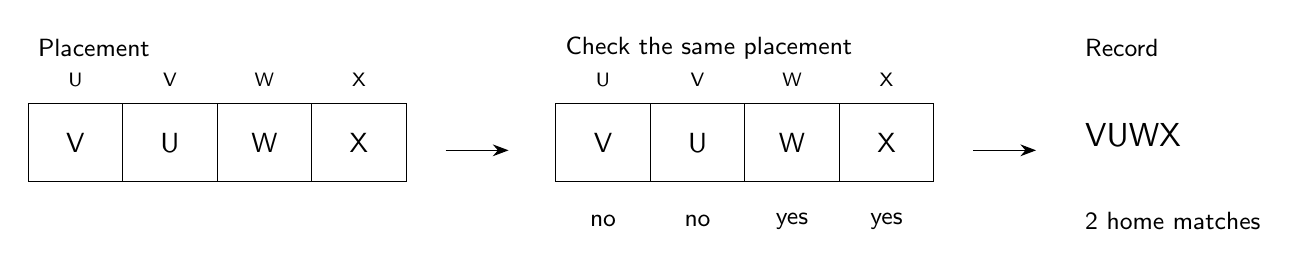
\begin{tikzpicture}[x=1mm,y=1mm]
  \node[anchor=west,font=\small] at (0,14) {Placement};
  \rowdraw{0}{7}{U,V,W,X}{V,U,W,X}
  \draw[-{Stealth[length=2mm]}] (53,1)--(61,1);
  \node[anchor=west,font=\small] at (67,14) {Check the same placement};
  \rowdraw{67}{7}{U,V,W,X}{V,U,W,X}
  \foreach \s/\x in {no/73,no/85,yes/97,yes/109}{\node[font=\small] at (\x,-8) {\s};}
  \draw[-{Stealth[length=2mm]}] (120,1)--(128,1);
  \node[anchor=west,font=\small] at (133,14) {Record};
  \node[anchor=west,font=\large] at (133,3) {VUWX};
  \node[anchor=west,font=\small] at (133,-8) {2 home matches};
\end{tikzpicture}
\end{center}

\problem{1}{Find every row of A, B, C with no home matches. Can a row of these three cards have exactly two home matches?}
\blankrows{5}{A,B,C}{3}
\vspace{8mm}
\worklines{2}

\nextpage{Grades 2--5}
One outcome card is one whole placement. It can belong to several groups at once. Group the outcome cards on the table.

\begin{center}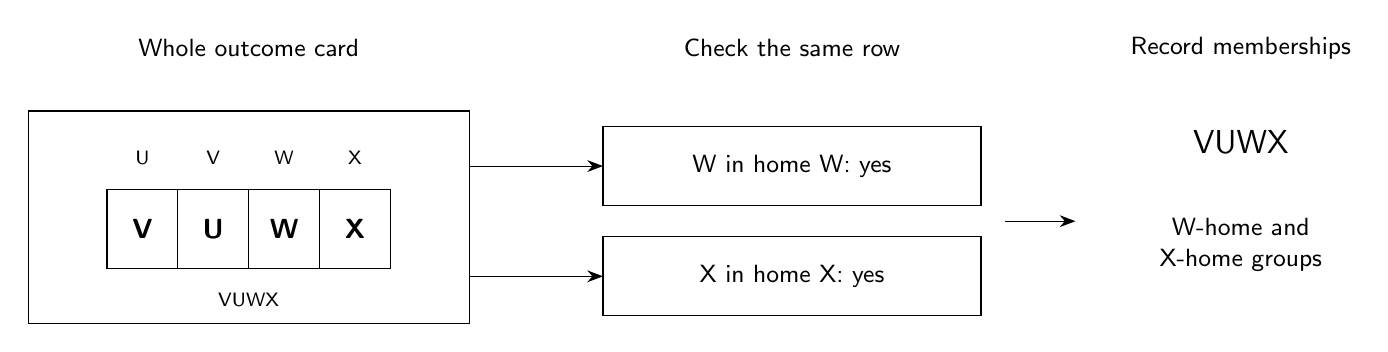
\begin{tikzpicture}[x=1mm,y=1mm]
  \node[font=\small] at (28,35) {Whole outcome card};
  \draw[thin] (0,0) rectangle (56,27);
  \foreach \h [count=\i from 0] in {U,V,W,X}{%
    \node[font=\scriptsize] at ({10+\i*9+4.5},21) {\h};
    \draw[thin] ({10+\i*9},7) rectangle ++(9,10);
  }
  \foreach \c [count=\i from 0] in {V,U,W,X}{%
    \node[font=\normalsize\bfseries] at ({10+\i*9+4.5},12) {\c};
  }
  \node[font=\scriptsize] at (28,3) {VUWX};
  \node[font=\small,align=center] at (97,35) {Check the same row};
  \draw[thin] (73,15) rectangle (121,25);
  \draw[thin] (73,1) rectangle (121,11);
  \node[font=\small] at (97,20) {W in home W: yes};
  \node[font=\small] at (97,6) {X in home X: yes};
  \draw[-{Stealth[length=2mm]}] (56,20)--(73,20);
  \draw[-{Stealth[length=2mm]}] (56,6)--(73,6);
  \draw[-{Stealth[length=2mm]}] (124,13)--(133,13);
  \node[font=\small] at (154,35) {Record memberships};
  \node[font=\large] at (154,23) {VUWX};
  \node[font=\small,align=center] at (154,10) {W-home and\\X-home groups};
\end{tikzpicture}\end{center}

\problem{2}{Use the six A--C outcome cards. Make one group with A in home A and another with B in home B. A card may belong to both groups. How many rows are outside both groups? C may stay home.}

A student counts $6-2-2=2$. Repair this count and show what went wrong.

\vspace{4mm}
\begin{center}\begin{tikzpicture}[x=1mm,y=1mm]
  \draw[rounded corners=3mm,thin] (0,0) rectangle (173,70);
\end{tikzpicture}\end{center}
\vspace{7mm}
\worklines{3}

\nextpage{Grades 3--5}
\problem{3}{Find every A--D row with no home matches. Make a catalog your table can check for repeated or missing rows.}
\blankrows{8}{A,B,C,D}{4}
\vspace{5mm}
\worklines{2}

\nextpage{Grades 3--5}
\problem{4}{Count the A--D rows with A away from home A and B away from home B. C and D may stay home. Use the 24 outcome cards to check the count $24-6-6$. How should the count be repaired?}
\vspace{4mm}
\begin{center}\begin{tikzpicture}[x=1mm,y=1mm]
  \draw[thin,rounded corners=3mm] (0,0) rectangle (173,95);
\end{tikzpicture}\end{center}
\vspace{8mm}
\worklines{4}

\nextpage{Grades 3--5}
\problem{5}{There are four home-groups: A at A, B at B, C at C, and D at D. Each contains six of the 24 A--D rows. A student tries $24-6-6-6-6$ to count the rows outside every group. Repair the count using overlaps.}

An overlap includes every row with the required matches, even when other cards are also home.

\vspace{3mm}
\begin{center}\begin{tikzpicture}[x=1mm,y=1mm]
  \draw[thin,rounded corners=3mm] (0,0) rectangle (173,97);
\end{tikzpicture}\end{center}
\vspace{4mm}
\worklines{3}

\nextpage{Grades 4--5}
\problem{6}{There are 120 A--E rows. Count those with no home matches by correcting overlaps of the five home-groups. Show why your correction keeps each wanted row once and removes every other row.}
\vspace{3mm}
\begin{center}\begin{tikzpicture}[x=1mm,y=1mm]
  \draw[thin,rounded corners=3mm] (0,0) rectangle (173,127);
\end{tikzpicture}\end{center}
\vspace{5mm}
\worklines{4}

\nextpage{Grades 4--5}
An arrow points from a card's letter to the home where that card sits.

\begin{center}\begin{tikzpicture}[x=1mm,y=1mm]
  \node[anchor=west,font=\small] at (0,28) {Placement};
  \rowdraw{0}{19}{P,Q,R,S,T}{Q,R,S,T,P}
  \draw[-{Stealth[length=2mm]}] (63,11)--(71,11);
  \node[font=\small,align=center] at (92,18) {P is in home T};
  \node[font=\large] at (92,8) {P $\longrightarrow$ T};
  \draw[-{Stealth[length=2mm]}] (115,11)--(123,11);
  \node[font=\small] at (151,28) {All arrows};
  \begin{scope}[shift={(151,5)}]\cyclefive{P,T,S,R,Q}{17}\end{scope}
\end{tikzpicture}\end{center}

\problem{7}{Keep D in home A. Find every A--D row with no home matches, and draw its arrows. Sort the rows into those with A in home D and those with A away from home D. What makes your list complete?}
\begin{center}\begin{tikzpicture}[x=1mm,y=1mm]
  \fourworkspace{36}{-33}
  \fourworkspace{127}{-33}
  \fourworkspace{36}{-110}
  \fourworkspace{127}{-110}
\end{tikzpicture}\end{center}
\worklines{2}

\nextpage{Grades 4--5}
Smaller arrow loops keep their remaining letters. These examples remove U, then can be read backward to restore U.

\begin{center}\begin{tikzpicture}[x=1mm,y=1mm]
  \node[font=\small] at (25,28) {Input};
  \node[font=\small] at (86,28) {Remove U};
  \node[font=\small] at (148,28) {Output};
  \begin{scope}[shift={(25,2)}]
    \node[circle,draw,minimum size=6mm,inner sep=0pt,font=\small] (p) at (-12,15) {P};
    \node[circle,draw,minimum size=6mm,inner sep=0pt,font=\small] (u) at (12,15) {U};
    \draw[-{Stealth[length=1.8mm]}] (p) to[bend left=18] (u);
    \draw[-{Stealth[length=1.8mm]}] (u) to[bend left=18] (p);
    \begin{scope}[shift={(0,-13)}]\cyclefour{Q,R,S,T}{13}\end{scope}
  \end{scope}
  \draw[-{Stealth[length=2mm]}] (48,0)--(57,0);
  \node[font=\small,align=center] at (86,0) {P and U point\\to each other.\\Remove both.};
  \draw[-{Stealth[length=2mm]}] (114,0)--(123,0);
  \begin{scope}[shift={(148,0)}]\cyclefour{Q,R,S,T}{17}\end{scope}

  \node[font=\small] at (25,-45) {Input};
  \node[font=\small] at (86,-45) {Remove U};
  \node[font=\small] at (148,-45) {Output};
  \begin{scope}[shift={(25,-70)}]\cyclesix{P,Q,R,S,T,U}{19}\end{scope}
  \draw[-{Stealth[length=2mm]}] (48,-70)--(57,-70);
  \node[font=\small,align=center] at (86,-70) {T $\to$ U $\to$ P\\becomes\\T $\to$ P};
  \draw[-{Stealth[length=2mm]}] (114,-70)--(123,-70);
  \begin{scope}[shift={(148,-70)}]\cyclefive{P,Q,R,S,T}{18}\end{scope}
\end{tikzpicture}\end{center}

\problem{8}{Keep E in home A. Make every home-free A--E row in two families: A in home E, and A away from home E. How can each family be built from smaller home-free rows? Give constructions you can reverse.}
\vspace{4mm}
\worklines{4}

\nextpage{Grades 4--5}
\problem{9}{Choose one of homes A, B, C, D for E. Make a complete catalog of home-free A--E rows with E there. Pool the four catalogs to count all home-free A--E rows. Use the two families to give a counting rule for two or more distinct cards, and explain why each row is counted once.}
\blankrows{8}{A,B,C,D,E}{5}
\vspace{1mm}
\worklines{2}
\end{document}
